\section{Economics}

Miners are privileged actors who choose transactions to include
in the sidechain blocks.
In order to ensure honesty, there must be some method to punish
nefarious validators when cryptographically-verifiable malicious
behavior is observed.
Therefore, all miners are required to stake a certain amount of Ether
in a smart contract before being able to become a validator.
This ensures the desired Nash equilibrium: it is in the miner's
interest to correctly follow the procedure and receive compensation
rather than to deviate from it and lose significant stake.
This includes malicious behavior during the distributed key generation
procedure (for example, failing to correctly share a secret) as well
as when mining blocks (for example, signing two different proposals).
All cryptographically-verifiable malicious behavior will be validated
as such by an Ethereum smart contract.
We note that submitting a false accusation is malicious behavior
and will result in stake slashing.

In order to ensure security, we do not allow direct withdrawals
at this time; this is due to security concerns and complexities
of exit games.
In particular, there is the possibility miners could create tokens
out of thin air and then quickly move those tokens to the
Ethereum blockchain.
By not allowing for direct withdrawals, those tokens created out
of thin air cannot be removed.
Creating such tokens would be malicious behavior by a miner who would
then be punished accordingly.
If necessary, the sidechain may be reorganized to negate such
malicious behavior;
however, it is not possible to invalidate blocks on Ethereum once
they have been committed.
Thus, atomic swaps are safer than direct withdrawals in the context
of our security model and we take this approach.

We allow for deposits from Ethereum into the sidechain to occur
through direct exchange.
When a deposit occurs in the Ethereum MainNet, tokens are burned
in the Ethereum Chain and an equal number of tokens become available
after a minimum block wait time in the sidechain.

Miners are rewarded in two different ways.
The first way miners are rewarded is upon the completion of an epoch
when a snapshot is written into the Ethereum blockchain.
This incentivizes miners to mine blocks and have the system progress,
as mining more blocks will result in more rewards.
Snapshots occur at a fixed interval of sidechain blocks as well as
after a minimum required number of Ethereum blocks.

Validators are also rewarded for cleaning up stale state;
that is, when a DataStore has expired, the miner can delete the
DataStore and claim its deposit as a reward.
Both of these rewards are in the form of MadNet tokens.
This means that miners will be the source of token liquidity
within the system, as they are required to have an Ethereum account
as well as having a significant supply of tokens;
furthermore, they determine which transactions are included
in the blocks they propose and could include their atomic swaps.
In order to store data, MadNet tokens are required to be burned.
So long as the data exists, more tokens are burned to compensate
the miners for being required to store the data.

In order to establish value stability during the initial period of low
utilization, an incentivized mechanism of illiquidity has been
established.
This mechanism is designed to allow token holders to lock balances of
tokens into a smart contract that will return yield to the owner that
is expressed as a function of token utilization and the amount locked.

First, the amount of illiquid tokens is set.
From there, we divide these tokens into different tranches; each
tranche holds tokens for a predetermined time.
The longer holding requirements will result in a greater rate of return.
Should we determine that the system requires more tokens, tokens may be
released, starting with the lowest yield tranche and working toward the
highest yield.
A bonus will be paid for early release as specified in the smart
contract; the exact rate of return will be discussed below.
We expect the number of tokens required to follow a normal
distribution, so we use that to help distribute the tokens
appropriately in the tranches.
Below is a plot of the relative sizes of the tranches.
The exact number of tranches is yet to be determined but there is no
restriction on the allowable number.
In the plot below, the tranches will be released from left to right,
starting near 0 and ending near 1; see Fig.~\ref{fig:tranches}.
The specified rate of return will increase from left to right.

\begin{figure}
    \centering
    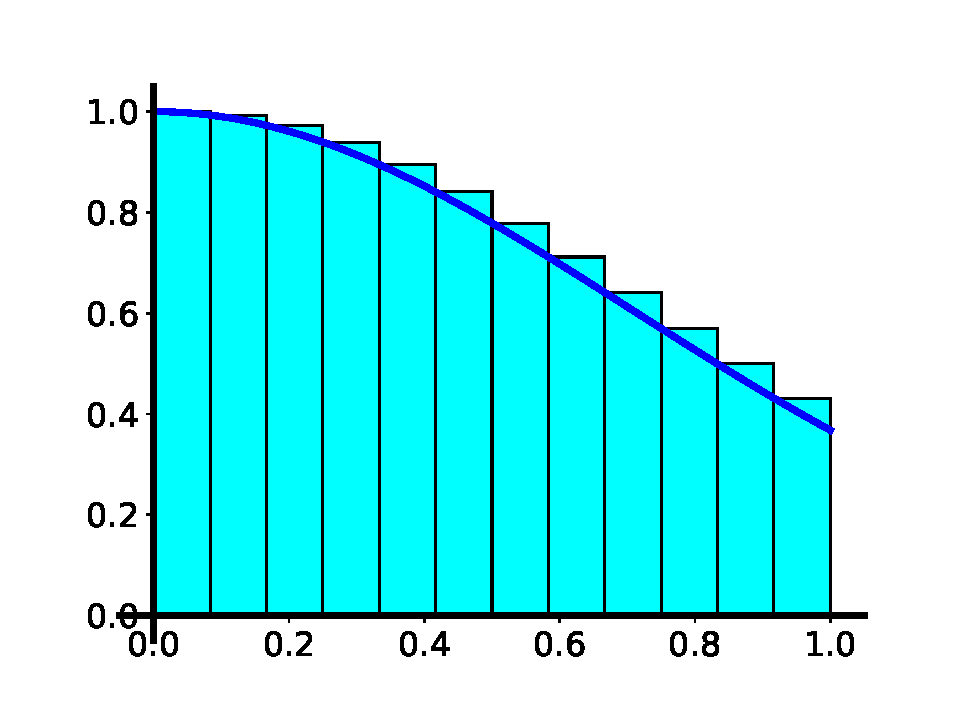
\includegraphics[scale=0.5]{figures/tranches_plot.pdf}
    \caption{Relative size of an potential set of tranches
        to incentize illiquidity.}
    \label{fig:tranches}
\end{figure}



A larger rate of return will occur should tokens need to be released
into the market sooner than anticipated.
The actual rate of return will be determined in relation to the
expected holding and will vary smoothly with respect to time (the
number of blocks); the maximum payout will be double the expected rate
of return.
All of this helps ensure a stable initial value for the token.
A plot of the rate of return is shown below.
Note the plot is the tokens paid out in addition to what was deposited.
Here, if the tokens are released at one-half the holding time, the rate
of return will be twice the agreed upon amount.
Similarly, if the tokens are released at the originally agreed upon
time, the rate of return will be the agreed upon amount (technically, a
slightly greater amount); see Fig.~\ref{fig:rate_of_return}.
Thus, if tokens are quickly released, there will be only a small
payout, but after an initial period of time, the rate of return will be
at least the specified amount.

\begin{figure}
    \centering
    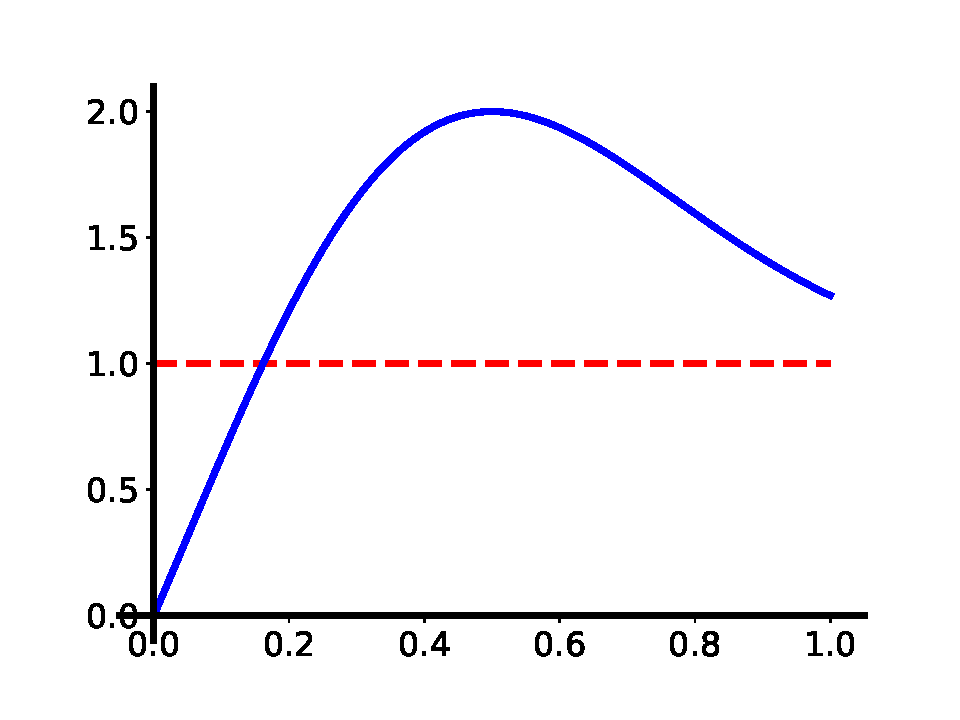
\includegraphics[scale=0.5]{figures/ror_plot.pdf}
    \caption{This plot shows how the specified rate of return will be
        multiplied by to show the actual rate of return.
        The maximum return occurs when the tokens in the tranche are
        released at one-half of the number of blocks they were originally
        held.
        This would occur because the system requires a large supply
        of tokens.}
    \label{fig:rate_of_return}
\end{figure}


